% -- Encoding UTF-8 without BOM
% -- XeLaTeX => PDF (BIBER)

\documentclass{cv-style}     % Add 'print' as an option into the square bracket to remove colours from this template for printing.

\setdefaultlanguage{french}
\sethyphenation{french}{} % Add words between the {} to avoid them to be cut

%----------------------------------------------------------------------------------------
%	Page layout
%----------------------------------------------------------------------------------------
\cvheadheight{3.5cm}
\cvasidewidth{4.7}
\cvasidevpos{3.5}
\cvmainwidth{11.5cm}
\geometry{left=6.4cm, top=2.5cm, right=1cm, bottom=1cm}

%----------------------------------------------------------------------------------------
%	Bibliography
%----------------------------------------------------------------------------------------
\usepackage[sectcntreset]{bibtopic}
\usepackage{natbib}
\bibliographystyle{bib/achemso_perso}
\AtBeginDocument{\nocite{achemso-control}}

%----------------------------------------------------------------------------------------
%	hyperlink setup
%----------------------------------------------------------------------------------------
\hypersetup{
    pdftitle=CV \textbar{} Laura Gomez,%
    pdfauthor=Laura Gomez
}

%----------------------------------------------------------------------------------------
%	Setup las updated text
%----------------------------------------------------------------------------------------
%\lastupdated{Mise à jour le \today}

%----------------------------------------------------------------------------------------
%	Add a few custom packages
%----------------------------------------------------------------------------------------
\usepackage{fontawesome}

\begin{document}

\header{Laura }{Gomez}{Chef de projet technique -- mécatronique et biomécanique}         % Your name
%\lastupdated

%----------------------------------------------------------------------------------------
%	SIDEBAR SECTION  -- In the aside, each new line forces a line break
%----------------------------------------------------------------------------------------

\begin{aside}
    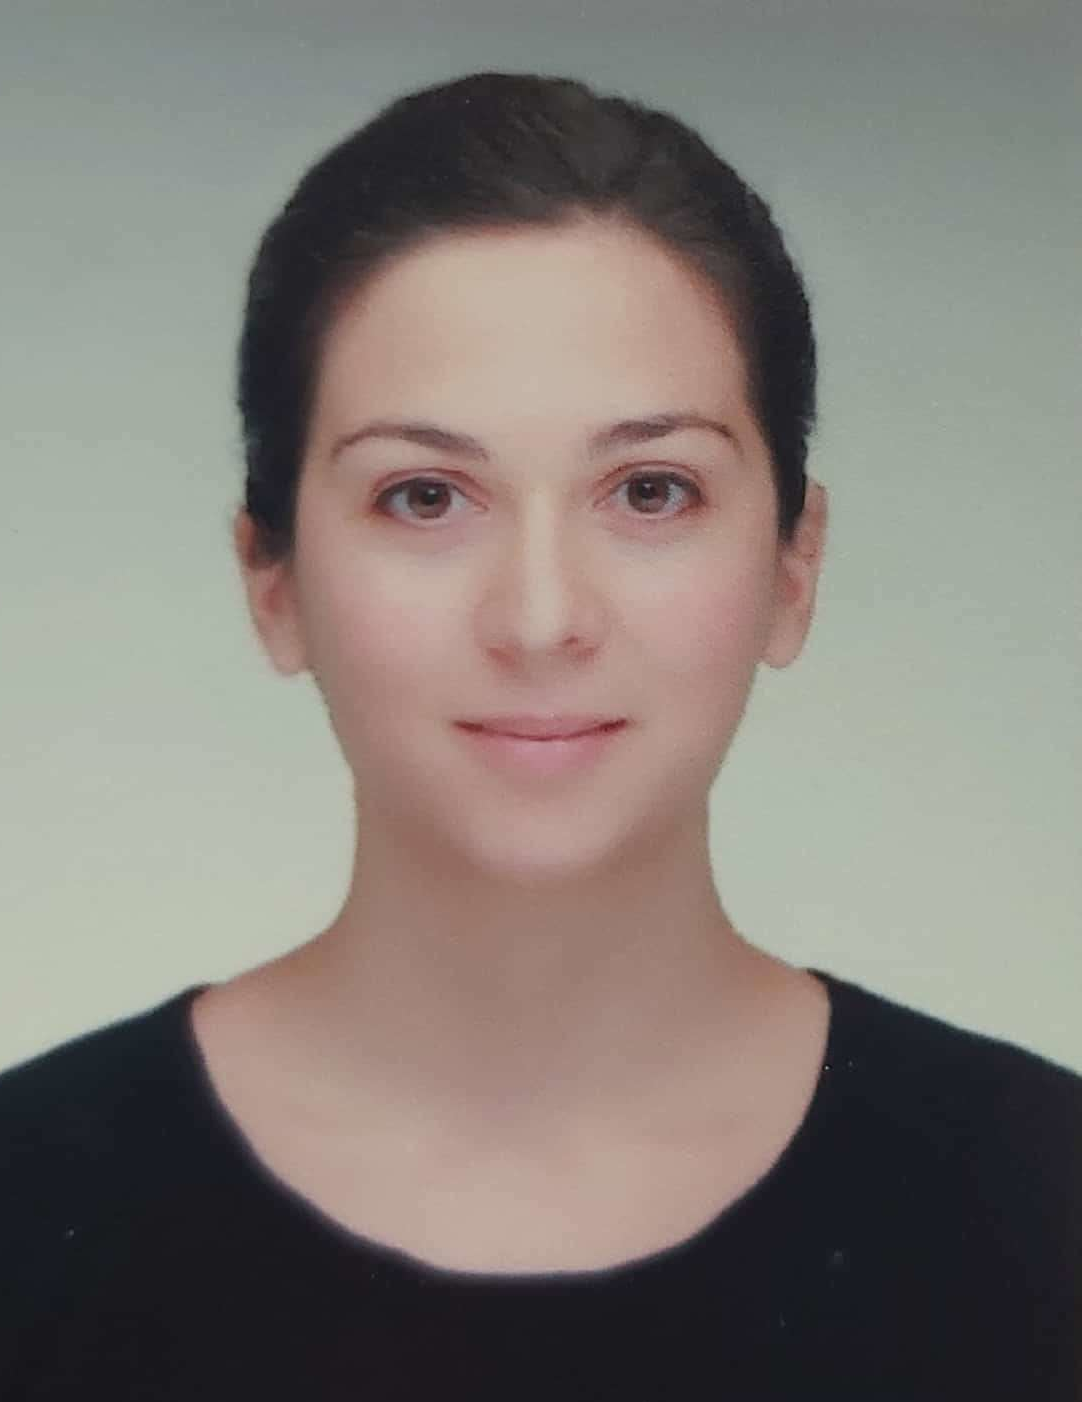
\includegraphics[width=.8\columnwidth]{img/LG}
    Disponibilité immédiate
    Permis B
    ~
    13 janvier 1989, France
    En concubinage
    %
    \section{Contact}
    laura-gomez@gmx.fr
    +33 7 70 49 23 44
    ~
    91 rue du Colonel Fabien
    92160 Antony
    France
    %
    \section{Gestion de projet}
    Microsoft Office
    ERP (Dolibarr, Sage)
    Gestion des exigences (DOORS, Reqtify)
    ~
    Rédaction brevet
    Suivi Certification CE
    %
    \section{Logiciel}
    C, Matlab
    Systèmes embarqués %(Arduino, Mbed)
    CAO %(Solidworks, Fusion360, OpenSim)
    Simulation multiphysique %(Flotherm)
    Conception Electronique %(Simulink, Labview, Zuken, Altium) 
    Outils d’étude du movement humain %(Nexus pour Vicon, MT Manager pour Xsens (centrales inertielles))
    %
    \section{Langues}
    Français 
    Anglais 
    Espagnol
    %
    \section{Soft Skills}
    Autonome et proactive
    Pensée analytique
    Bon esprit d'équipe
    %
\end{aside}

\section{Rés}{umé}

Mécatronicienne de formation, j’ai eu l’occasion de piloter le développement matériel et logiciel de nouveaux produits jusqu’à leur industrialisation, ainsi que de produits déjà existants afin de les adapter aux besoins spécifiques de clients. 
Assurer une bonne communication entre toutes les parties prenantes internes et externes concernées, afin de respecter les délais et  la qualité de la prestation est également l’une de mes priorités. 
Je participe finalement à la coordination du projet jusqu’à la commercialisation, y compris les phases d’industrialisation, le marquage réglementaire et la fourniture de la documentation. 
J’aime être proactive dans l’amélioration de la méthodologie de développement de produits et j’aimerais également un jour pouvoir partager mes acquis en créant et dispensant une formation sur les produits aux équipes internes et aux clients externes. 

\section{Experience}{ Professionnelle}

\begin{entrylist}
%------------------------------------------------
\entry
  {depuis 2010~}
  {Université de Pau et des Pays de l'Adour}
  {Pau, France}
  {\jobtitle{Maître de conférences}\\
   Chimie théorique et simulation numérique.
   Surface, interface et réactivité.}
%------------------------------------------------
\entry
  {2009--2010}
  {CEA - DAM}
  {Bruyères le châtel, France}
  {
  \jobtitle{Chercheur-ingénieur}\\
  Développement et implémentation d'un modèle mésoscopique pour l'étude de la propagation
  d'ondes de chock réactives dans un système hétérogène.
  }
%------------------------------------------------
\entry
  {2006--2009}
  {Université Paris-Sud 11}
  {Orsay, France}
  {
  \jobtitle{Allocataire de recherche, moniteur}\\
  Étude théorique de processus photophysiques dans les protéines fluorescentes.
  }
%------------------------------------------------
\end{entrylist}

%----------------------------------------------------------------------------------------
%	EDUCATION SECTION
%----------------------------------------------------------------------------------------

\section{Form}{ation}

\begin{entrylist}
%--------------------------------------G----------
\entry
{2013-2015}
{Master d'ingénierie biomédical {\normalfont spécialité biomécanique}}
{BME et Arts et Métiers}
{}
%------------------------------------------------
\entry
{2008-2013}
{Ecole d'ingénieur en mécatronique {\normalfont spécialité robotique et simulation}}
{ISTY - UVSQ}
{6 mois en Corée à l'Université Ajou}
%------------------------------------------------
% \entry
% {2003-2004}
% {Licence de chimie-physique}
% {Université Paris-Sud 11}
% {Mention TB}
% %------------------------------------------------
% \entry
% {2003-2006}
% {Magistère de Physico-Chimie Moléculaire}
% {Université Paris-Sud 11 -- ENS Cachan}
% {}
% %------------------------------------------------
% \entry
% {2001-2003}
% {CPGE {\normalfont PCSI-PC}}
% {Lycée François Arago, Perpignan}
% {}
\end{entrylist}

%----------------------------------------------------------------------------------------
%	OTHER QUALIFICATIONS SECTION
%----------------------------------------------------------------------------------------

% \section{Publications}{ significatives}

% \nocite{vallverdu2016, guille2015, Guille2014, Martin2012, Maillet2011, Vallverdu2010}
% \begin{btSect}{bib/articles}
%     \btPrintCited
% \end{btSect}

%----------------------------------------------------------------------------------------
%	INTERESTS SECTION
%----------------------------------------------------------------------------------------

% \section{Centres d'intérêts}
%   \vspace{-0.2cm}
%
% \textbf{Informatiques:} Outils numériques et pédagogiques, programmation,
% communautée open-source.\\
% \textbf{Personnels:} Membre au CA de l'association APNEE, rugby, guitare, flûte.

%----------------------------------------------------------------------------------------

\end{document}
